%【紙面設定】
%b4,横書き,2段
\documentclass[paper=b4j,landscape,twocolumn,fleqn]{jlreq}
\special{papersize=\the\paperwidth,\the\paperheight}
\setlength{\columnseprule}{0.4pt}
\pagestyle{empty}
\usepackage[margin=8truemm]{geometry}
\usepackage[dvipdfmx]{graphicx}
\usepackage{amsmath}
\usepackage{tikz}
\ModifyHeading{section}{lines=1,before_space=6pt,after_space=0pt}
\setlength{\parskip}{0pt}
\setlength{\jot}{3pt}

%【本文】
\begin{document}
\normalsize
\section{覚えるべき三角形の図示 解答}
\begin{align*}
&1.\ 30^\circ\text{-}60^\circ\text{-}90^\circ\text{ の辺比 }1:\sqrt{3}:2\\[0.45em]
&2.\ 45^\circ\text{-}45^\circ\text{-}90^\circ\text{ の辺比 }1:1:\sqrt{2}\\[0.45em]
&3.\ \text{最短辺}=1\Rightarrow (1,\sqrt{3},2)\\[0.45em]
&4.\ \text{斜辺}=1\Rightarrow \left(\frac{\sqrt{2}}{2},\frac{\sqrt{2}}{2},1\right)\\[0.45em]
&5.\ \sin30^\circ=\frac12,\ \cos30^\circ=\frac{\sqrt3}{2},\ \sin45^\circ=\cos45^\circ=\frac{\sqrt2}{2},\ \sin60^\circ=\frac{\sqrt3}{2},\ \cos60^\circ=\frac12\\[0.45em]
&6.\ \tan30^\circ=\frac{1}{\sqrt3},\ \tan45^\circ=1,\ \tan60^\circ=\sqrt3
\end{align*}
\textbf{考え方}\
基準三角形の辺比を先に固定する。$30^\circ\text{-}60^\circ\text{-}90^\circ$ は $1:\sqrt3:2$、$45^\circ\text{-}45^\circ\text{-}90^\circ$ は $1:1:\sqrt2$。\\
\textbf{途中式（代表例）}
\begin{align*}
&\sin30^\circ=\frac{\text{対辺}}{\text{斜辺}}=\frac12,\ \cos30^\circ=\frac{\sqrt3}{2}\\
&\tan60^\circ=\frac{\text{対辺}}{\text{隣辺}}=\frac{\sqrt3}{1}=\sqrt3
\end{align*}
\textbf{図説（覚えるべき2つの三角形）}
\begin{center}
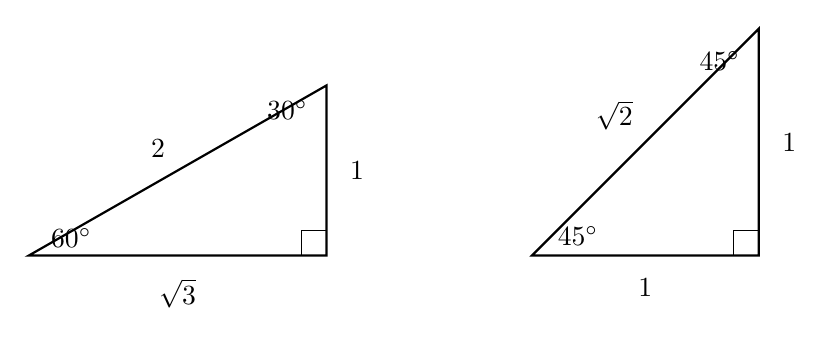
\begin{tikzpicture}[scale=0.9]
	% 30-60-90
	\coordinate (A) at (0,0);
	\coordinate (B) at (4.2,0);
	\coordinate (C) at (4.2,2.4);
	\draw[thick] (A)--(B)--(C)--cycle;
	\draw (3.85,0) -- (3.85,0.35) -- (4.2,0.35);
	\path (A)--(B) node[midway,below=5pt] {$\sqrt3$};
	\path (B)--(C) node[midway,right=5pt] {$1$};
	\path (A)--(C) node[midway,above left=1pt] {$2$};
	\path (C) ++(-0.55,-0.35) node {$30^\circ$};
	\path (A) ++(0.6,0.25) node {$60^\circ$};

	% 45-45-90
	\coordinate (D) at (7.1,0);
	\coordinate (E) at (10.3,0);
	\coordinate (F) at (10.3,3.2);
	\draw[thick] (D)--(E)--(F)--cycle;
	\draw (9.95,0) -- (9.95,0.35) -- (10.3,0.35);
	\path (D)--(E) node[midway,below=5pt] {$1$};
	\path (E)--(F) node[midway,right=5pt] {$1$};
	\path (D)--(F) node[midway,above left=1pt] {$\sqrt2$};
	\path (F) ++(-0.55,-0.45) node {$45^\circ$};
	\path (D) ++(0.65,0.28) node {$45^\circ$};
\end{tikzpicture}
\end{center}

\newpage
\section{直角三角形の比 解答}
\begin{align*}
&1.\ 2,\ 2\sqrt3,\ 4\\[0.45em]
&2.\ 4,\ 4\sqrt3,\ 8\\[0.45em]
&3.\ 6,\ 6,\ 6\sqrt2\\[0.45em]
&4.\ 30^\circ\text{側}=3,\ \text{斜辺}=6\\[0.45em]
&5.\ 60^\circ\text{側}=5\sqrt3,\ \text{斜辺}=10\\[0.45em]
&6.\ \text{もう1辺}=4,\ \text{斜辺}=4\sqrt2
\end{align*}
\textbf{考え方}\
与えられた辺を基準比に対応させ、倍率をかける。\\
\textbf{途中式（代表例）}
\begin{align*}
&1.\ 30\text{-}60\text{-}90\text{比 }1:\sqrt3:2\text{ で最短辺 }2\Rightarrow \times2\\
&\quad (2,2\sqrt3,4)\\
&3.\ 45\text{-}45\text{-}90\text{比 }1:1:\sqrt2,\ \text{斜辺 }6\sqrt2\Rightarrow \text{倍率 }6\\
&\quad (6,6,6\sqrt2)
\end{align*}

\newpage
\section{三角比 解答}
\begin{align*}
&1.\ \cos30^\circ=\frac{\sqrt3}{2},\ \cos45^\circ=\frac{\sqrt2}{2},\ \cos60^\circ=\frac12\\[0.45em]
&2.\ \sin30^\circ=\frac12,\ \sin45^\circ=\frac{\sqrt2}{2},\ \sin60^\circ=\frac{\sqrt3}{2}\\[0.45em]
&3.\ \tan30^\circ=\frac{1}{\sqrt3},\ \tan45^\circ=1,\ \tan60^\circ=\sqrt3\\[0.45em]
&4.\ \text{底辺}=4\sqrt3,\ \text{高さ}=4\\[0.45em]
&5.\ \text{底辺}=5,\ \text{高さ}=5\sqrt3\\[0.45em]
&6.\ \text{斜辺}=6\sqrt2,\ \text{高さ}=6
\end{align*}
\textbf{考え方}\
$\sin\theta=\frac{\text{高さ}}{\text{斜辺}},\ \cos\theta=\frac{\text{底辺}}{\text{斜辺}},\ \tan\theta=\frac{\text{高さ}}{\text{底辺}}$ を使う。\\
\textbf{途中式（代表例）}
\begin{align*}
&4.\ \theta=30^\circ,\ \text{斜辺 }8\Rightarrow \text{高さ}=8\sin30^\circ=8\cdot\frac12=4\\
&\quad \text{底辺}=8\cos30^\circ=8\cdot\frac{\sqrt3}{2}=4\sqrt3\\
&6.\ \theta=45^\circ,\ \tan45^\circ=1\Rightarrow \text{高さ}=\text{底辺}=6\\
&\quad \text{斜辺}=\sqrt{6^2+6^2}=6\sqrt2
\end{align*}

\newpage
\section{ラジアン 解答}
\begin{align*}
&1.\ 30^\circ=\frac\pi6,\ 45^\circ=\frac\pi4,\ 60^\circ=\frac\pi3,\ 90^\circ=\frac\pi2\\[0.45em]
&2.\ \frac\pi6=30^\circ,\ \frac\pi4=45^\circ,\ \frac\pi3=60^\circ,\ \frac\pi2=90^\circ\\[0.45em]
&3.\ \cos\frac\pi3=\frac12,\ \sin\frac\pi6=\frac12,\ \tan\frac\pi4=1\\[0.45em]
&4.\ \text{底辺}=4\sqrt3,\ \text{高さ}=4\\[0.45em]
&5.\ \text{底辺}=2\sqrt2,\ \text{高さ}=2\sqrt2\\[0.45em]
&6.\ \text{斜辺}=6,\ \text{高さ}=3\sqrt3
\end{align*}
\textbf{考え方}\
$180^\circ=\pi$ を基準に変換。辺計算は度数法と同じで角度表記だけが違う。\\
\textbf{途中式（代表例）}
\begin{align*}
&1.\ 60^\circ=\frac{60}{180}\pi=\frac\pi3\\
&2.\ \frac\pi4=\frac{180}{4}^\circ=45^\circ\\
&6.\ \theta=\frac\pi3(=60^\circ),\ \cos\theta=\frac12=\frac{\text{底辺}}{\text{斜辺}}=\frac{3}{\text{斜辺}}\\
&\quad \text{斜辺}=6,\ \text{高さ}=6\sin\frac\pi3=6\cdot\frac{\sqrt3}{2}=3\sqrt3
\end{align*}

\newpage
\section{単位円の三角比 解答}
\begin{align*}
&1.\ \sin\theta=\frac{\sqrt3}{2},\ \cos\theta=\frac12,\ \tan\theta=\sqrt3\\[0.45em]
&2.\ \sin\theta=\frac{\sqrt2}{2},\ \cos\theta=\frac{\sqrt2}{2},\ \tan\theta=1\\[0.45em]
&3.\ \sin\theta=\frac{\sqrt3}{2},\ \cos\theta=-\frac12,\ \tan\theta=-\sqrt3\\[0.45em]
&4.\ \cos\theta=\pm\frac{2\sqrt2}{3},\ \tan\theta=\pm\frac{\sqrt2}{4}\\[0.45em]
&5.\ \sin\theta=\frac{\sqrt{15}}{4},\ \tan\theta=\sqrt{15}\\[0.45em]
&6.\ \sin\theta=\frac{2\sqrt5}{5},\ \cos\theta=\frac{\sqrt5}{5}
\end{align*}
\textbf{考え方}\
単位円では $\cos\theta=x,\ \sin\theta=y,\ \tan\theta=\frac{y}{x}$。また $\sin^2\theta+\cos^2\theta=1$ を使う。\\
\textbf{途中式（代表例）}
\begin{align*}
&3.\ P\left(-\frac12,\frac{\sqrt3}{2}\right)\Rightarrow \cos\theta=-\frac12,\ \sin\theta=\frac{\sqrt3}{2}\\
&\quad \tan\theta=\frac{\sin\theta}{\cos\theta}=\frac{\sqrt3/2}{-1/2}=-\sqrt3\\
&6.\ \tan\theta=2\Rightarrow \sin\theta=2\cos\theta\\
&\quad (2\cos\theta)^2+\cos^2\theta=1\Rightarrow 5\cos^2\theta=1\\
&\quad \cos\theta=\frac{\sqrt5}{5},\ \sin\theta=\frac{2\sqrt5}{5}
\end{align*}
\textbf{図説（単位円と三角比）}
\begin{center}
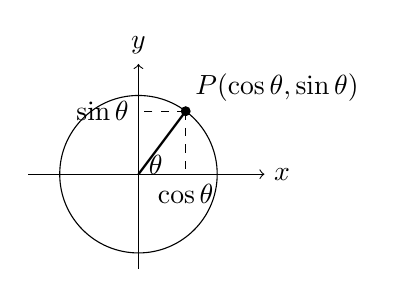
\begin{tikzpicture}[scale=1.0]
	\draw[->] (-1.4,0)--(1.6,0) node[right] {$x$};
	\draw[->] (0,-1.2)--(0,1.4) node[above] {$y$};
	\draw (0,0) circle (1);
	\coordinate (P) at (0.6,0.8);
	\fill (P) circle (1.8pt) node[above right] {$P(\cos\theta,\sin\theta)$};
	\draw[thick] (0,0)--(P);
	\draw[dashed] (P)--(0.6,0) node[below] {$\cos\theta$};
	\draw[dashed] (P)--(0,0.8) node[left] {$\sin\theta$};
	\node at (0.22,0.12) {$\theta$};
\end{tikzpicture}
\end{center}

\newpage
\section{三角比の総合 解答}
\begin{align*}
&1.\ \frac{1+\sqrt3}{2}\\[0.45em]
&2.\ \frac12\\[0.45em]
&3.\ \frac{\sqrt3}{2}\\[0.45em]
&4.\ \sqrt3+2\\[0.45em]
&5.\ 1\\[0.45em]
&6.\ \cos\theta=\frac45,\ \tan\theta=\frac34
\end{align*}
\textbf{考え方}\
既知角は値を直接代入。未知角は恒等式と象限条件で符号を決める。\\
\textbf{途中式（代表例）}
\begin{align*}
&4.\ 2\cos\frac\pi6+4\sin\frac\pi6=2\cdot\frac{\sqrt3}{2}+4\cdot\frac12=\sqrt3+2\\
&6.\ \sin\theta=\frac35,\ 0<\theta<\frac\pi2\\
&\quad \cos\theta=\sqrt{1-\sin^2\theta}=\sqrt{1-\frac{9}{25}}=\frac45\\
&\quad \tan\theta=\frac{\sin\theta}{\cos\theta}=\frac{3/5}{4/5}=\frac34
\end{align*}
\end{document}


